\documentclass{article}
\usepackage{amsmath, physics}
\usepackage[UTF8]{ctex}
\usepackage{graphicx}
\usepackage{float}

\begin{document}

\section*{2021年攻读博士学位研究生招生考试试卷}
\section*{考试科目名称:普通物理(满分100分)}

\section*{一、简答题(30分)}

\begin{enumerate}
  \item[1.] (10分) 质点系的动能定理、动量定理、角动量定理及质心运动定理推导
  
  \textbf{解答:}
  \begin{itemize}
    \item 动能定理:$\sum W_{\text{外力}} + \sum W_{\text{内力}} = \Delta E_k$
    \item 动量定理:$\sum \mathbf{F}_{\text{外力}} = \dv{\mathbf{P}}{t}$
    \item 角动量定理:$\sum \mathbf{M}_{\text{外力}} = \dv{\mathbf{L}}{t}$
    
    由动量定理推导质心运动定理:
    $$
    \mathbf{P} = m\mathbf{v}_c \Rightarrow \dv{\mathbf{P}}{t} = m\mathbf{a}_c = \sum \mathbf{F}_{\text{外力}}
    $$
    质心位置定义式:
    $$
    \mathbf{r}_c = \frac{\sum m_i\mathbf{r}_i}{\sum m_i}
    $$
  \end{itemize}

  \item[2.] (5分) 气体平衡状态特征及分子运动
  
  \textbf{解答:}
  平衡态特征:宏观性质稳定,无物质/能量流动;微观上分子持续热运动,碰撞频率分布稳定。

  \item[3.] (5分) 导体表面电场与电荷面密度关系
  
  \textbf{解答:}
  取高斯面(圆柱形):
  $$
  \oint \mathbf{E} \cdot d\mathbf{A} = \frac{\sigma \Delta S}{\varepsilon_0} \Rightarrow E = \frac{\sigma}{\varepsilon_0}
  $$
  即$\mathbf{E} = \dfrac{\sigma}{\varepsilon_0}\mathbf{n}$

  \item[4.] (5分) 单缝衍射图样变化分析
  
  \textbf{解答:}
  \begin{itemize}
    \item (1) 所有明纹变宽,条纹间距增大
    \item (2)--(4)见图片
    \begin{figure}[H]
        \centering
        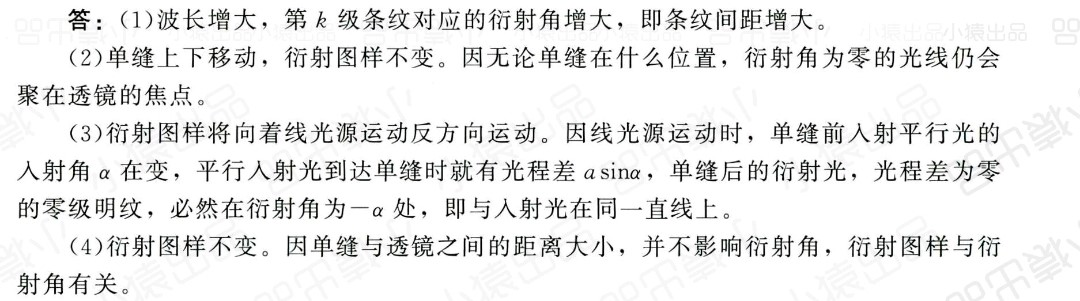
\includegraphics[width=1.3\linewidth]{Screenshot_20250416_215216.jpg}
    \end{figure}
  \end{itemize}

  \item[5.] (5分) 电子动能计算
  
  \textbf{解答:}
  \begin{align*}
    \lambda &= \frac{h}{p} \Rightarrow p = \frac{h}{\lambda} \\
    E_k &= \frac{p^2}{2m_e} = \frac{(6.63\times10^{-34})^2}{2\times9.11\times10^{-31}\times(550\times10^{-9})^2} \\
    &\approx 8.9\times10^{-20}\ \text{J} \approx 0.56\ \text{eV}
  \end{align*}
\end{enumerate}

\section*{二、计算题(70分)}

\begin{enumerate}
  \item[1.] (10分) 导体球电势为零条件
  \begin{figure}[H]
      \centering
      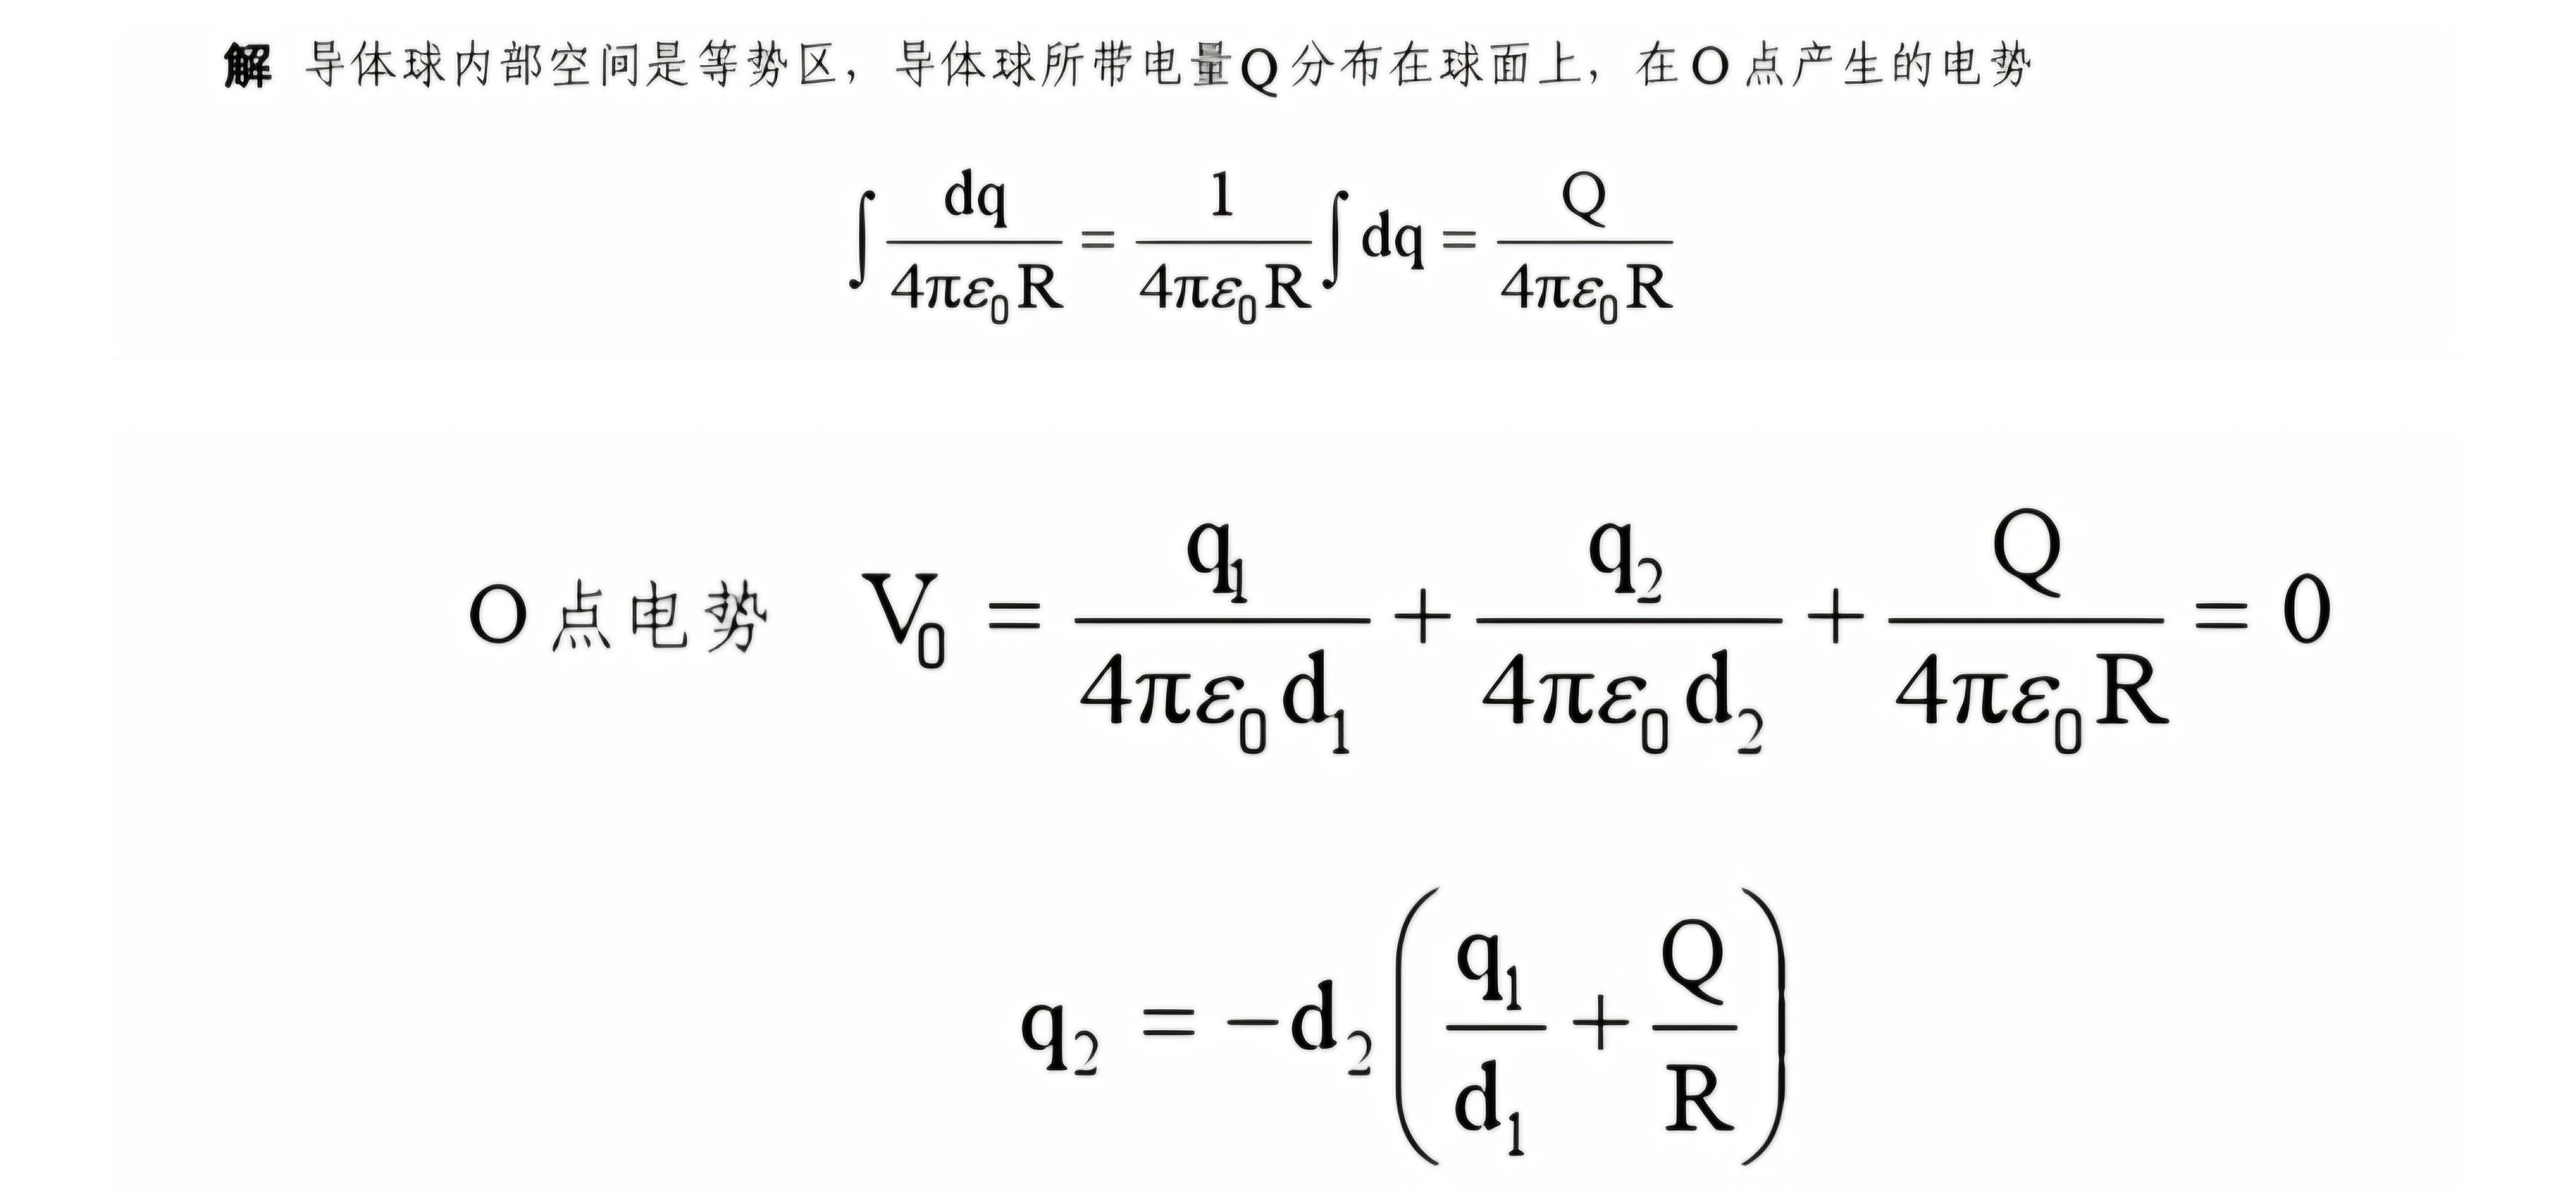
\includegraphics[width=1.4\linewidth]{Screenshot_20250414_090905.jpg}
  \end{figure}
  \textbf{解答:错误}
  电势叠加:
  $$
  \frac{1}{4\pi\varepsilon_0}\left( \frac{Q}{R} + \frac{q_1}{d} + \frac{q_2}{d} \right) = 0
  $$
  解得:
  $$
  q_2 = -\left( Q\frac{d}{R} + q_1 \right)
  $$

  \item[2.] (20分) 导体棒运动分析
  
  \textbf{解答:}
  \begin{itemize}
    \item 1) 运动方程:
    $$
    m\dv{v}{t} = -\frac{B^2l^2(v-v')}{2R}
    $$
    由对称性得速度关系:
    $$
    v(t) = \frac{v_0}{2}(1 + e^{-\frac{B^2l^2}{mR}t})
    $$
    
    \item 2) 最大间距增量:
    $$
    \Delta x_{\text{max}} = \int_0^\infty v(t)dt = \frac{mRv_0}{B^2l^2}
    $$
  \end{itemize}
\end{enumerate}
\subsection*{第三题(20分)}
1摩尔单原子分子理想气体,从初态 $(p_0, V_0)$ 经过准静态压缩过程到达终态 $(8p_0, \frac{1}{4}V_0)$。

\begin{enumerate}
  \item[(1)] (10分) 假设全过程每个无穷小过程中气体对外作功 $dA$ 与吸热量 $dQ$ 之比 $\frac{dA}{dQ} = \beta$ 为常量,求 $\beta$
  
  \item[(2)] (10分) 计算气体的熵增量 $\Delta S$
\end{enumerate}

\subsection*{解答}
\begin{figure}[H]
    \centering
    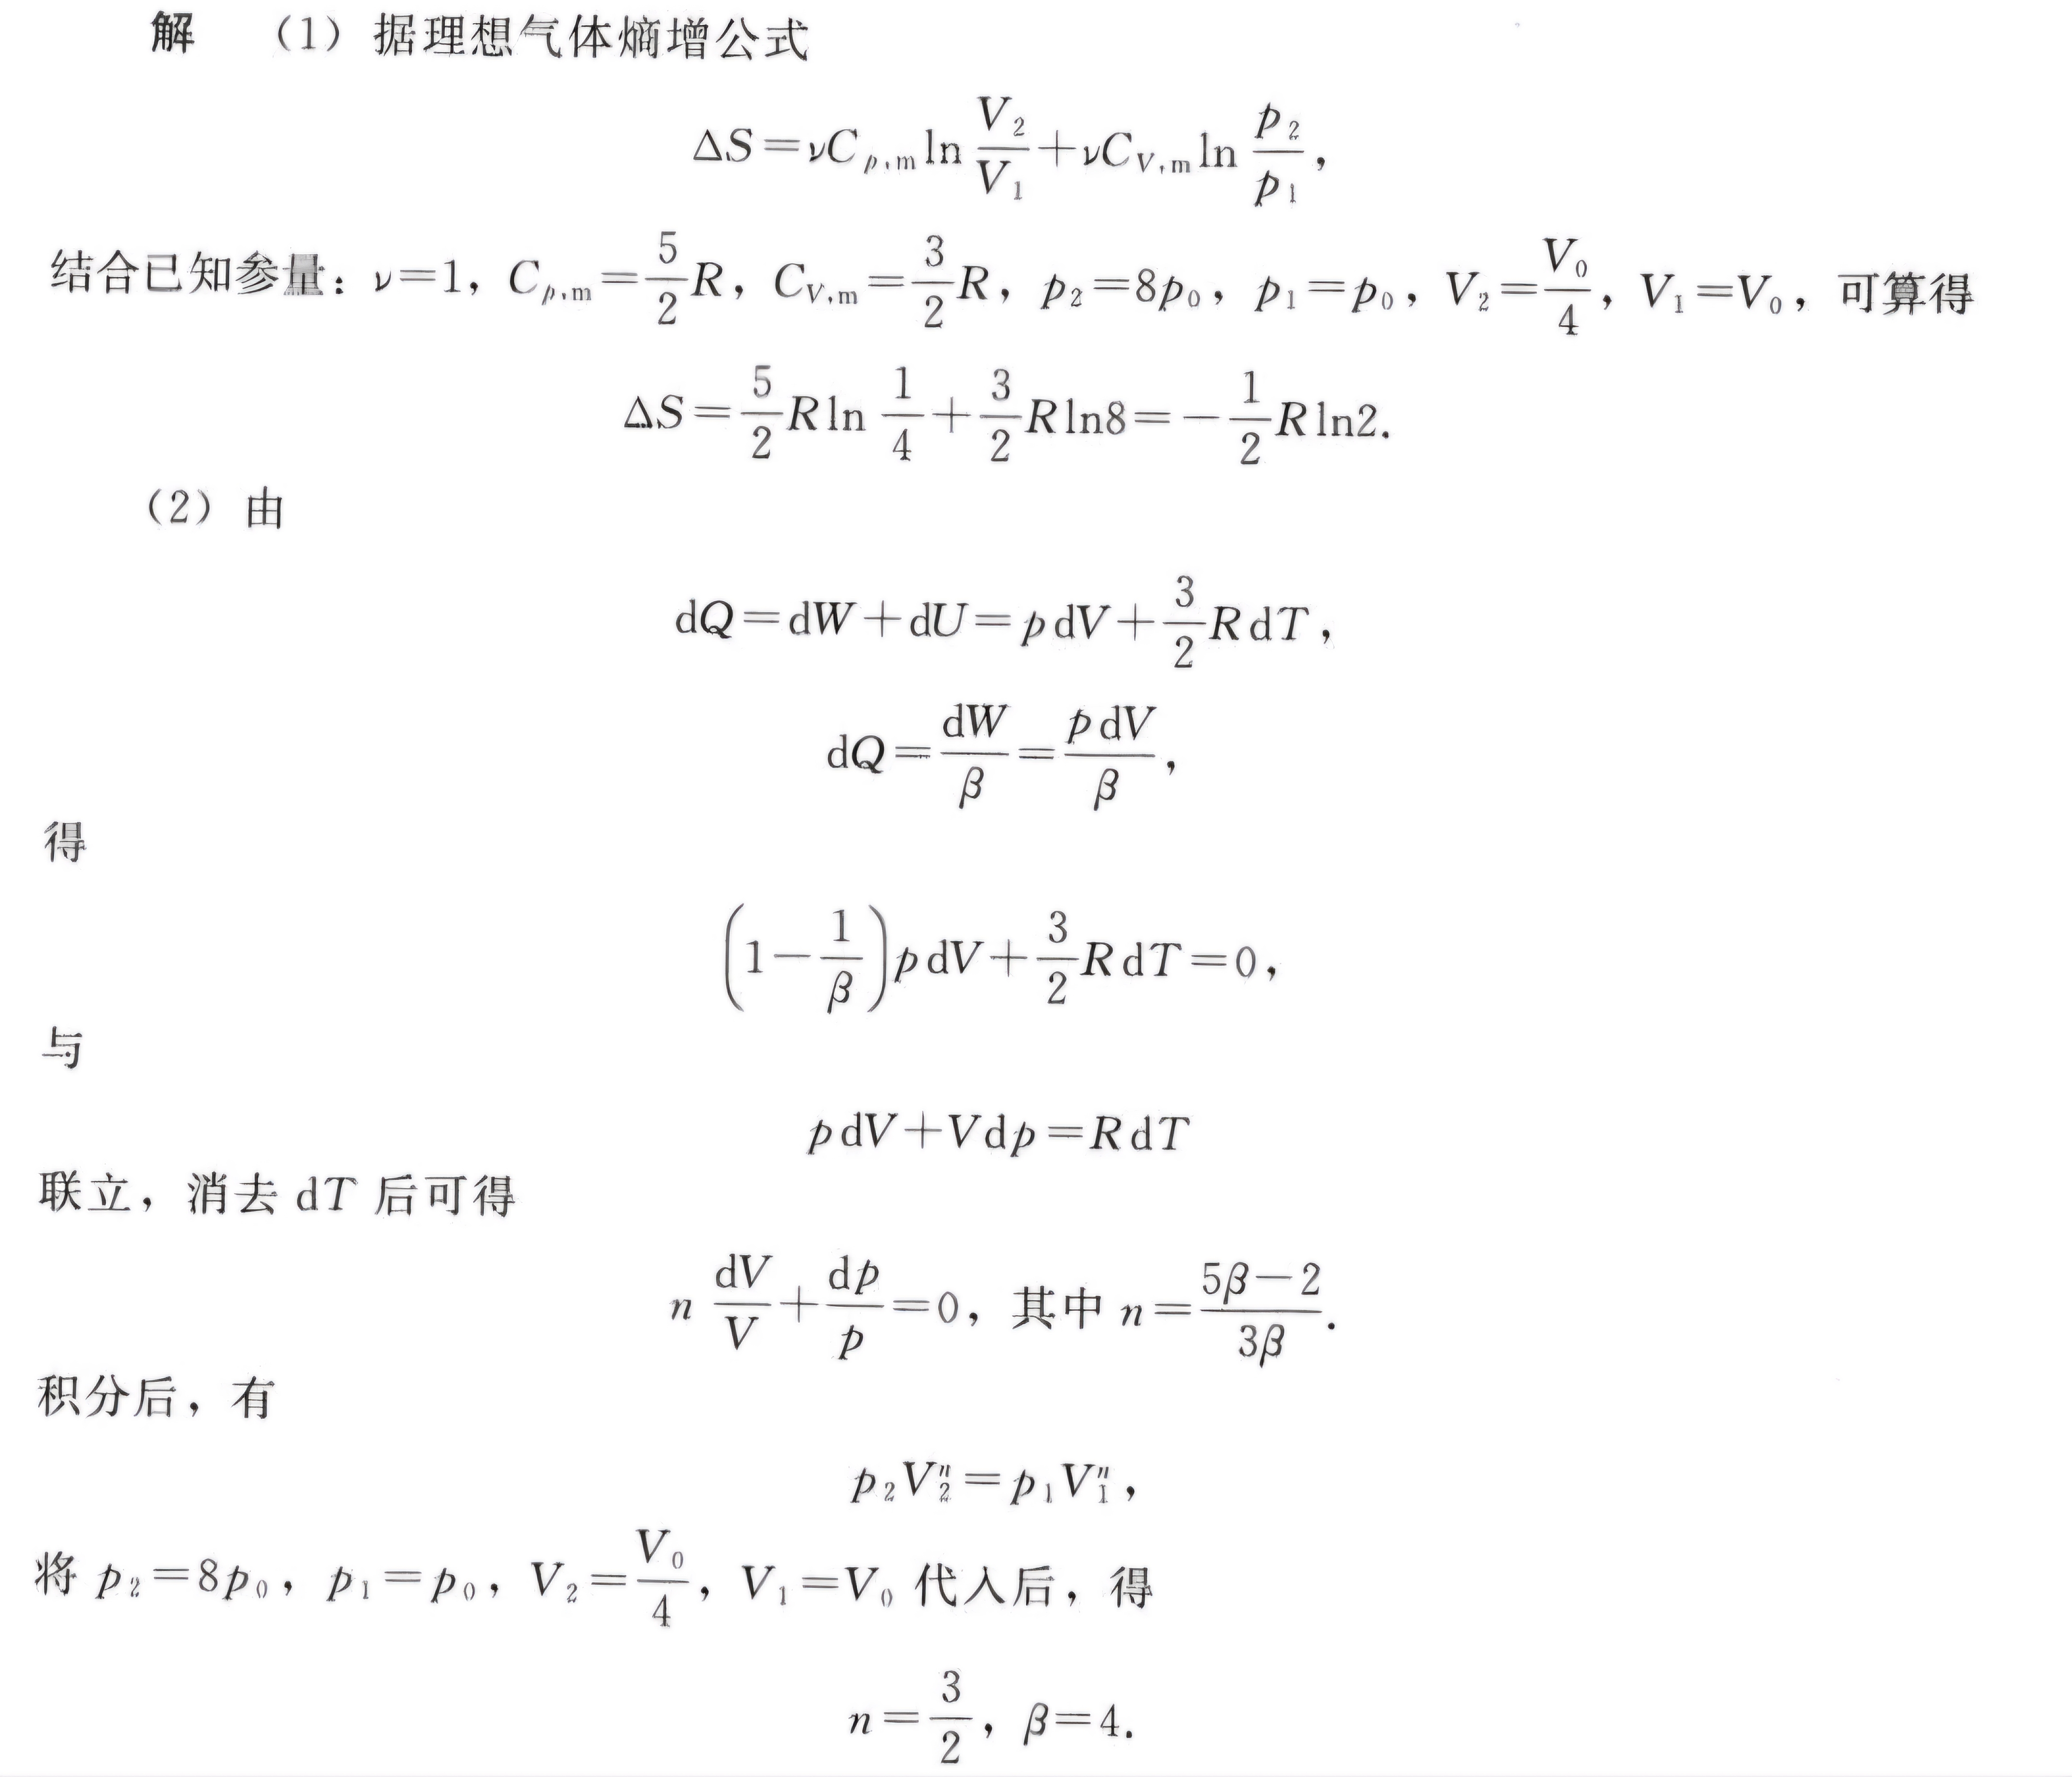
\includegraphics[width=1.3\linewidth]{Screenshot_20250416_225431.jpg}
\end{figure}

% 第四题
\subsection*{第四题(20分)有错}
杨氏实验中,波长为500nm的单色光垂直照射双缝,屏幕上产生干涉条纹。在上方狭缝后放置$n=1.5$的介质。

\begin{enumerate}
  \item[(1)] (6分) 条纹间距变化及中央条纹移动方向
  \item[(2)] (8分) 介质厚度计算(中央明纹移至原第三级暗纹)
  \item[(3)] (6分) 反射镜交点处的干涉类型
\end{enumerate}

\subsection*{解答}

\item[(1)] \textbf{条纹变化分析}
\begin{enumerate}
在杨氏双缝实验中,当在上面的狭缝后放置折射率n=1.5的介质时,需要考虑光程差的变化对干涉条纹的影响。

1. **光程差的变化**:上面狭缝的光程增加了(n-1)t(t为介质的厚度),而下面狭缝的光程不变。这导致两束光的光程差增加了一个固定值(n-1)t。

2. **干涉条件**:新的光程差为d sinθ + (n-1)t,其中d为双缝间距,θ为衍射角。干涉条件变为d sinθ + (n-1)t = mλ(m为整数)。

3. **条纹位置**:新的明纹位置满足y = [mλ - (n-1)t] D/d,其中D为双缝到屏幕的距离。相邻明纹的间距Δy由相邻m值的差决定,即Δy = λD/d,与原来的条纹间距公式相同。

4. **波长影响**:光通过介质后波长会变短为λ/n,但在离开介质进入空气后,波长恢复为原来的λ。因此,两束光在屏幕上的干涉仍然使用空气中的波长λ进行计算。

5. **结论**:虽然光程差的固定增加会导致整个干涉图样平移,但相邻条纹的间距由波长λ、双缝间距d和屏幕距离D决定,这些参数未改变,因此条纹间距不变。

最终答案:不变
\end{enumerate}
\begin{enumerate}
    在杨氏双缝实验中,当在上面的狭缝后放置折射率为 \( n = 1.5 \) 的介质时,中央条纹的位置会发生变化。以下是具体分析:

1. **光程差的变化**  
   - 上面狭缝的光程增加了 \( \Delta L = (n-1)t \),其中 \( t \) 为介质厚度。
   - 新的总光程差为:  
     \[
     \text{光程差} = \text{几何路径差} + (n-1)t
     \]
   - 原中央条纹对应光程差为零的位置,但插入介质后,需满足新的平衡条件:  
     \[
     \text{几何路径差} = -(n-1)t
     \]

2. **几何路径差的调整**  
   - 假设双缝 \( S_1 \)(上)和 \( S_2 \)(下)竖直排列。当观察点 \( P \) **上移**时,\( S_2 \) 到 \( P \) 的几何路径比 \( S_1 \) 到 \( P \) 的路径更长(如图)。  
   - 因此,新的中央条纹需满足:  
     \[
     S_2 \text{到} P \text{的几何路径} - S_1 \text{到} P \text{的几何路径} = (n-1)t
     \]
   - 这一条件要求 \( P \) **上移**,以增大 \( S_2 \) 的路径并减小 \( S_1 \) 的路径,从而抵消介质引入的光程差。

3. **结论**  
   由于介质导致上方光程增加,中央条纹需向**上移动**以补偿光程差,使总光程差为零。

最终答案:  上移
\end{enumerate}
  
  \item[(2)] \textbf{介质厚度计算}
  \begin{align*}
    \text{第三级暗纹条件} &\quad \delta = (n-1)t = (2m+1)\frac{\lambda}{2} \\
    \text{取}m=2 &\quad t = \frac{5\lambda}{2(n-1)} = \frac{5 \times 500\text{nm}}{2(0.5)} = 2500\text{nm} = 2.5\mu m
  \end{align*}
  
  \item[(3)] \textbf{反射镜干涉分析}
  \begin{itemize}
    \item 反射镜引入半波损失,等效光程差$\delta = \frac{\lambda}{2}$
    \item 交点在原零级位置,现满足相消干涉条件,为暗纹
  \end{itemize}

\end{document}